%% !TEX root = ../../handbook-physics.tex
%%!TEX TS-program = pdflatex
%%!TEX encoding = UTF-8 Unicode

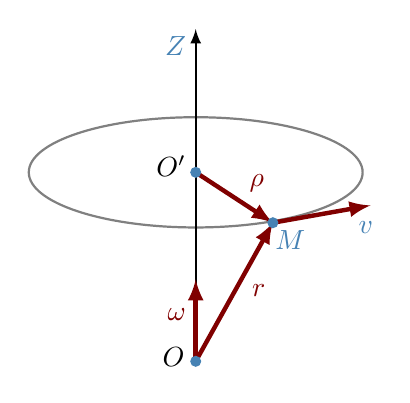
\begin{tikzpicture}[line cap=round,line join=round,scale=2]
\draw [rotate around={0.:(0.,2.)},thick,color=gray] (0.,2.) ellipse (1.06cm and 0.35cm);
\draw [thick,-latex] (0.,0.80)-- (0.,2.91);
\draw [ultra thick,Maroon,-latex] (0.,0.80)-- (0.49,1.68);
\draw [ultra thick,color=Maroon,-latex] (0.,2.)-- (0.49,1.68);
\draw [ultra thick,color=Maroon,-latex] (0.49,1.68)-- (1.11,1.79);
\draw [ultra thick,color=Maroon,latex-] (0.,1.32)-- (0.,0.80);
\draw (0,1.1) node [left,Maroon]{$\pmb{\omega}$};
\draw (0.28,2.05) node[anchor=north west,Maroon] {$\pmb{\rho}$};
\fill [fill=SteelBlue] (0.,0.80) circle (1pt);
\draw[] (-0.14,0.83) node {$O$};
\draw[color=SteelBlue] (0,2.8) node [left]{$Z$};
\fill [fill=SteelBlue] (0.49,1.68) circle (1pt);
\draw[color=SteelBlue] (0.6,1.57) node {$M$};
\draw[color=Maroon] (0.4,1.25) node {$\vb{r}$};
\fill [SteelBlue] (0.,2.) circle (1.0pt);
\draw[] (0,2.04) node[left] {$O'$};
\draw[color=SteelBlue] (1.08,1.65) node {$\vb{v}$};

\end{tikzpicture}
